\chapter{ANGULAR MOTION OF THE INTERFEROMETER MIRRORS}

For light to resonate in the interferometer, the mirrors need to point at one another and remain stationary with respect to this pointing. It is necessary to actively align the mirrors for several reasons:
\begin{itemize}
\item to find the optimal DC alignment of the interferometer \vspace{-10 pt}
\item to suppress any motion that results from external disturbances \vspace{-10 pt}
\item to counteract a high power static instability
\end{itemize}
There are 16 angular degrees of freedom that need to be sensed and controlled, making the ASC one of the most complex interferometer subsystems. This chapter presents the ASC design, and discusses the causes of mirror angular displacement and the effects of residual mirror motion on the interferometer. 



% normalize out seismic motion for wfs on / wfs off residual motion comparison

% how low can you go before it falls apart? valera and kate tried this
% out--find in elog

% RF offsets changing 

% possible in test runs to inc. hard/soft modes to 3
% hz, higher than ever before; but operationally, need lower. talk to
% matt and lisa to make sure to handle things politically correctly.

% calculate time-lag as cavity light responds to mirror displacements --> damping from RP





\section{Tolerance for Angular Motion}
\label{sec:tolerance}
%\textcolor{blue}{Make this section correct! power fluctuations only couple quadratically (bi-linearly) to DARM, but the contrast defect thing is \emph{indistinguishable} from gravitational waves. the A2L should still be emphasized.}


% Unlike DARM where the uncontrolled length displacement is what matters, it's the controlled  motion of the mirrors that matters for angular displacement. Too much residual motion, and both the lever arm effect and power fluctuations create noise in DARM. To prevent angular mirror motion from creating length displacements, the mirrors must not move more than $10^{-8}$ rad rms and the beam spots no more than 1 mm rms, as The residual motion must be held below 

Besides allowing the interferometer to be in a locked state, minimal motion of the mirrors is necessary to achieve the highest possible sensitivity to strain. The requirements for how much motion is tolerable stem from two effects of misalignment that directly couple to strain sensitivity: failure to achieve maximum power gain, and angle to length coupling. The misalignment tolerances are dictated by what is necessary to prevent the strain sensitivity of the perfectly aligned interferometer from degrading by more than 0.5\% in the detection band of 40-7000~Hz \cite{Fritschel1997Alignment}.

Because the strain sensitivity is proportional to the power at the beam splitter (see Eq.~\ref{eq:SNL}), a decrease in circulating power directly results in a decrease of shot-noise-limited DARM. Furthermore, differing power fluctuations in the two arm cavities results in a changing contrast defect, a difference in the amount of light returning from one arm compared to the other. A changing contrast defect creates power fluctuations at the AS port, making it indistinguishable from gravitational waves. Also, the DC power of the contrast defect contributes to increasing the shot noise noise-floor. Excessive fluctuations in the power recycling cavity makes for inconsistent signal to noise ratios for the signals that depend on sideband power. To maintain a power buildup within 1\% of maximum, the core optics must have an angular displacement of less than $10^{-8}$ rad rms with respect to the cavity axis \cite{ISCGroup1998ASC}. The derivation of power buildup as a function of mirror angle displacement is found in Appendix \ref{sec:cavitypower}.

Another deleterious effect of poor alignment is angle to length coupling. 
When the beam is located a distance $x$  away from the center of the mirror, an
angular displacement of the mirror $\theta$ about its center results in a path
length change of the beam
\begin{equation}
\Delta{L} = x \theta
\end{equation}
which has a direct impact on DARM. Therefore, the alignment specifications must include not only tolerable levels of angular motion, but requirements for the physical centering of the beam spots on the mirrors. As detailed in Ref. \cite{ISCGroup1998ASC}, the beams must be centered on the core optics within 1~mm. At DC, for x ~=~1 mm and $\theta = 10^{-7}$ rad, $\Delta{L} = 10^{-10}$ m which is four orders of magnitude below the DARM rms of $10^{-6}$ m. 
%\textcolor{blue}{Convolve my bsm spectra and residual mirror motion spectra to show example.}




\section{Sources of Angular Mirror Motion}
There is a continuous stream of changing torque inputs to the mirrors that cause them to twist and turn in pitch and in yaw. Some torque inputs exist regardless of the state of the interferometer, while others are a direct consequence of the control systems. The primary torque inputs are introduced here, and further discussion of some of them is found later in the chapter. The list includes:
\begin{itemize}
\item ground motion \vspace{-10pt} 
%\item seismic isolation \vspace{-10pt} 
\item coil actuators (length to angle) \vspace{-10pt}
\item noise impression from the angular control system \vspace{-10pt}
\item radiation pressure
\end{itemize}

%\textcolor{blue}{say something about seismometer feed-forward signals. say something about imperfect HEPI pos actuation}



\subsection{Ground Motion} 
\label{sec:oplevspectra}
The most egregious of these torque inputs is ground motion that makes its way through the multiple stages of seismic isolation to the mirror suspensions and thence to the mirrors. Ground motion is the only source of angular motion that is present regardless of the state of interferometer operation. An example of the shape and amount of angular motion experienced by the core optics due to seismic noise during a relatively quiet seismic time is shown in Figure \ref{fig:seismicMirror}.\footnote{These spectra include the effect of local velocity damping because the optical levers are always on. See Section~\ref{sec:suspension}.}. The rms mirror motion is of the order $10^{-7}$ rad. This is the motion that needs to be controlled interferometrically.

\begin{figure}
\begin{centering}
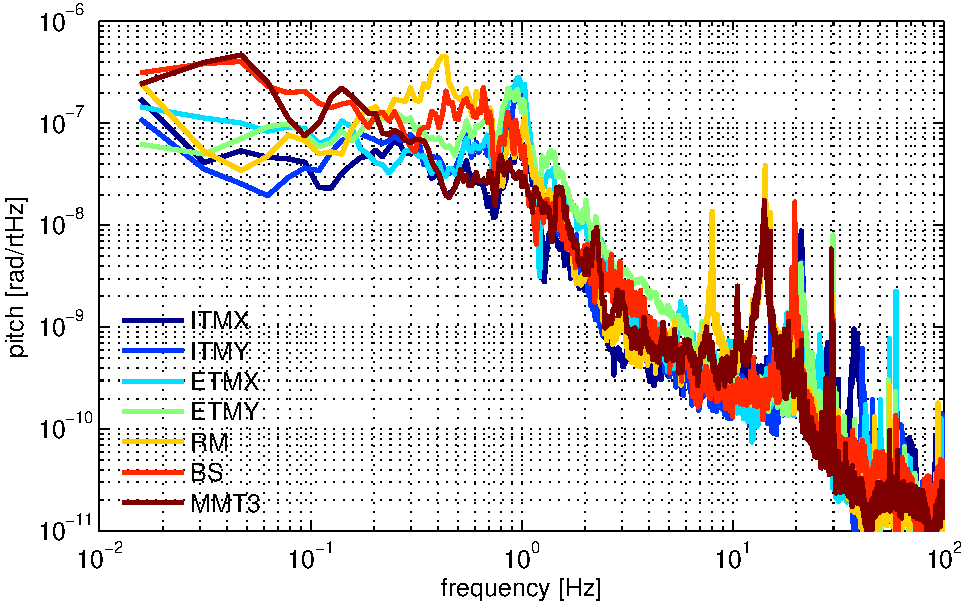
\includegraphics[width=1.0\columnwidth]{figures/seismic_mirrormotion.pdf}
\caption[Typical angular motion of the core suspended mirrors in the
  absence of interferometric control]{Typical angular motion of the core suspended mirrors in the 
  absence of interferometric control. Velocity damping provided by the
  OSEMs and the optical levers is present. Once the interferometer is locked, the OSEM damping is turned off. Ground motion at the time of this measurement is shown in Figure \ref{fig:seismic_nolock}.}
\label{fig:seismicMirror}
\end{centering}
\end{figure}

% Take a model of the optical lever open loop gains and a spectrum of
% optical lever error signal at a time when the interferometer is
% unlocked, but optical levers are on to calculate the background mirror
% motion due to seismic noise. Show the effect at a select few different
% times of day, probably for just one mirror. Write this section once I
% see what I have to present.

I obtained these spectra using the optical levers as witnesses of the mirror motion, which in turn is expected to come from the ground's motions. The optical lever signal, may, however, be contaminated by optical lever sensing (electronics) noise or acoustic couplings. It is therefore informative to embark on a study of how much of the optical lever spectra are in fact due to ground motion. 

I used a method of Wiener filtering \cite{Wiener1975Extrapolation} to show that the motion of Figure~\ref{fig:seismicMirror}, indeed originates primarily from the ground. The Wiener filter is the best estimate of the contribution of one signal to another. The contributions of the three seismometers to each large optic optical lever are shown in Figure~\ref{fig:OLcontributions}. We see that the optical lever signals are almost entirely explained by ground motion, with the notable exceptions being a peak between 3 and 4~Hz for ITMY, and 0.3 and 0.7~Hz for the RM, and broadband extra motion for the BS.

Furthermore, the relative magnitudes of the contributions from the
three seismometers make sense. Greater than 1~Hz, coherence is
greatest with the nearest seismometer, and less than 1~Hz,
seismometers contribute more equally (except for the ITMs, which are
everywhere very coherent with the corner station seismometer).

\begin{figure}
\begin{centering}
\subfigure{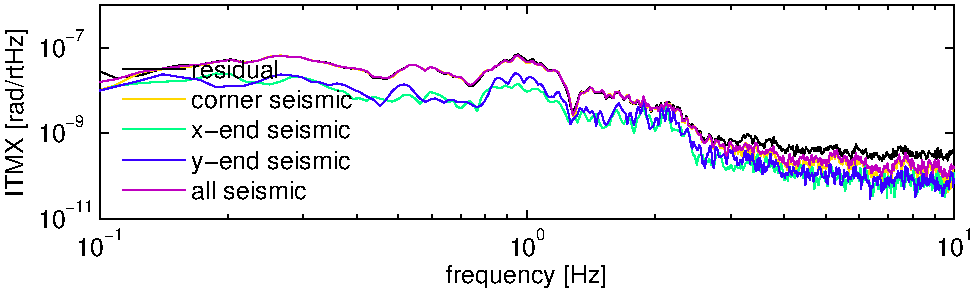
\includegraphics[width=1.0\textwidth]{figures/nolockIX.pdf}}
\subfigure{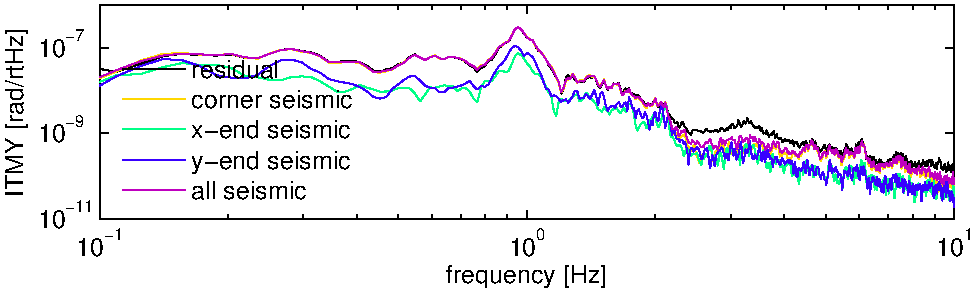
\includegraphics[width=1.0\textwidth]{figures/nolockIY.pdf}}
\subfigure{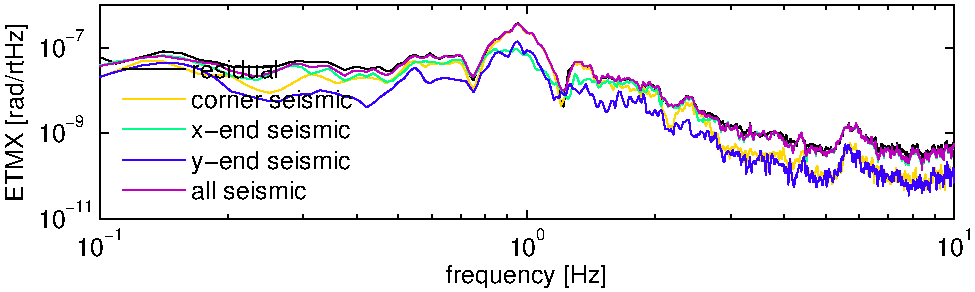
\includegraphics[width=1.0\textwidth]{figures/nolockEX.pdf}}
\subfigure{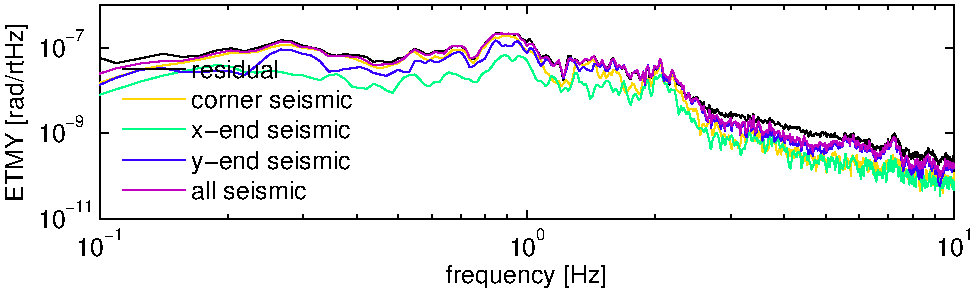
\includegraphics[width=1.0\textwidth]{figures/nolockEY.pdf}}
\caption[Contribution of seismic noise to optical lever error
signal]{Contribution of seismic noise to optical lever error signal
  (called residual). The interferometer was unlocked and optical lever
  and OSEM AC damping present.}
\label{fig:OLcontributions}
\end{centering}
\end{figure}

\begin{figure}
\begin{centering}
\subfigure{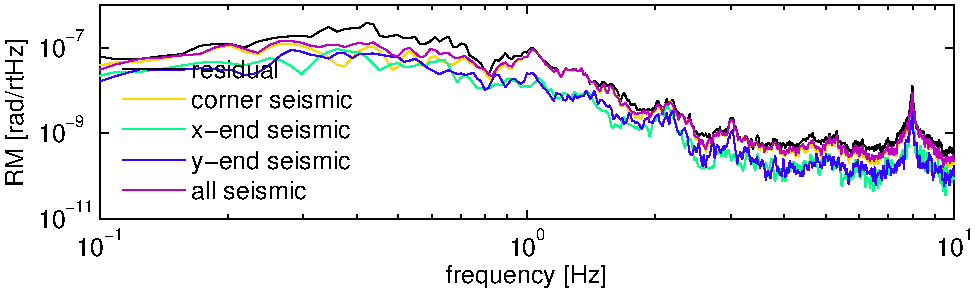
\includegraphics[width=1.0\textwidth]{figures/nolockRM.pdf}}
\subfigure{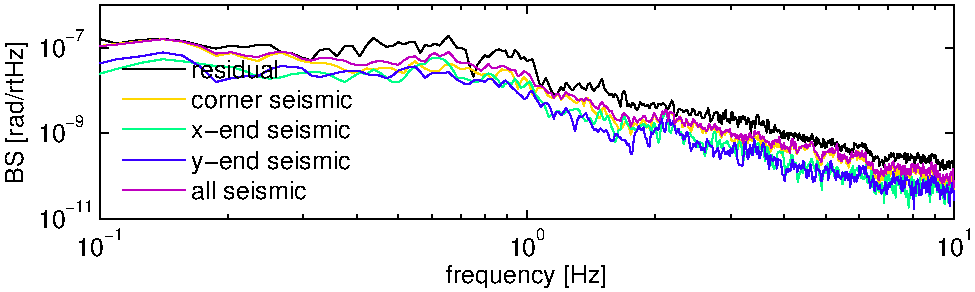
\includegraphics[width=1.0\textwidth]{figures/nolockBS.pdf}}
\subfigure{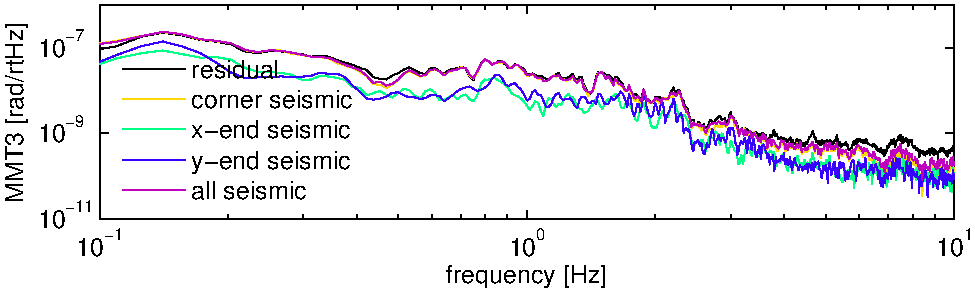
\includegraphics[width=1.0\textwidth]{figures/nolockMMT3.pdf}}
Figure~\ref{fig:OLcontributions} continued.
\end{centering}
\end{figure}




% \subsubsection{Seismic isolation}
% Although the multiple layers of seismic isolation serve to make interferometer operation possible \textcolor{blue}{write something better!}, minor imperfections in their implementation can result in them serving as coupling mechanisms to mirror angle. The path from ground to mirror can be broken into two distinct parts: HEPI + stack position to angle, and suspension position to angle. The seismic tables (HEPI at LLO) are actively actuated upon in position, ie. for the tidal servo. Any position to angle coupling will twist the table. The suspension 


% \subsubsection{Seismometers}
% The seismometers are sensitive to six degrees of freedom: x, y, z, and rotation about x, y, and z. Ideally, they are set up to only measure ground motion in x, y, and z, but the signals may be contaminated by some tilt as well. \textcolor{blue}{???}




\subsection{Coil Actuators} 
\label{sec:L2A}
Imperfections in the forces applied by the actuators on the rear of the test masses can convert piston (pure translation) drives into torque. The lengths of the cavities are carefully controlled (that's what we strive to be most sensitive to!) and any imbalances between the four electromagnets on a single mirror will create a coupling from length drive to angle (L2A). This effect is measurable, and then is carefully tuned out through selecting appropriate digital gains for each of the coils. Relative gain variation is 10\% of average. The ability to tune the gains perfectly is limited and the residual length to angle coupling is about 1\%. For the typical rms length drive of 1~\micronspace on a core optic and OSEMs separated by a distance of $\sqrt{2} R$ where $R$ is the radius of the optic, the 1\% L2A coupling results in a $10^{-8}$ radian displacement: 
\begin{equation} 
\theta = \frac{0.01 * 10^{-6} \mbox{ m}}{\sqrt{2} * 0.125 \mbox{ m}} \approx 10^{-8} \mbox{ rad}.  
\end{equation}

% Maybe include a figure that takes a typical length control spectrum signal to an optic and multiply by the above factors to show spectrum of angular motion induced by 1\% L2A.


\subsection{Noise from Angular Control}
The angular control system, which strives to counteract the above torque inputs to reduce angular motion, introduces angular mirror motion itself. The primary way it contributes noise is through imperfect sensing of the angular displacements. The alignment is also under-controlled, which ends up allowing the control system to impress input beam motion on the mirrors. These issues are explained in more detail in Section~\ref{sec:ASClimits}.


\subsection{Radiation Pressure} 
\label{sec:rp_intro}
Radiation pressure creates a torque when the beam impinges the mirror
off-center. The force on the mirror due to radiation pressure is
derived from the change in momentum of a photon upon reflection off
the mirror and results in:
\begin{equation}
F_{rp} = \frac{2 P} {c}
\end{equation}
where $P$ is the power of the light reflected by the mirror and $c$ is the
speed of light. Because the beam of photons strikes the mirror
perpendicular to its surface, the torque exerted on a mirror due to
radiation pressure is
\begin{equation}
\tau_{rp} = \frac{2 P x} {c}
\label{eq:tau_rp}
\end{equation}
where $x$ is the distance of the beam from the mirror's center of mass. For a 40~kW beam 1~mm off-center, the torque is on the order of $10^{-7}$ Nm, yielding an angular displacement of the order $10^{-7}$ rad as determined by the pendulum torque to angle transfer function. Refer to Section~\ref{sec:pendTF}.

Amongst the various torque inputs, radiation pressure plays a unique role in mirror motion because the torque it exerts depends on the angles of the mirrors. A result of the geometric coupling between beam displacements and mirror angles, radiation pressure therefore acts as an angular spring. It is best treated not as an external torque, but as a modification to the pendulum torque to angle transfer function. Chapter~\ref{ch:eigenmodes} dedicates a discussion to the physics of radiation pressure torques. In all, radiation pressure shapes the angular dynamics of the mirrors in LIGO and plays an important role in the design of an angular control system.






\section{The Mirror as a Torsion Pendulum}
\label{sec:pendTF}
In order to design a control system that reduces the angular motion of the interferometer mirrors to the levels necessary for stable interferometer operation and minimal impact on strain sensitivity, the angular response of the mirrors to external torque must be fully understood. A model of the mirror's torque to angle transfer function is thus required. To start, the mirrors in LIGO may be regarded as torsion pendula. The mirror may twist an angle $\theta$ about a horizontal axis passing through its center of mass to create motion in \emph{pitch} and about a vertical axis passing through its center of mass to create a motion in \emph{yaw}.

The angular equation of motion of the mirror is governed by the sum of
all torques on the mirror. First, let's consider the most simplistic
scenario where there is only a pendulum restoring torque
$\tau_p=-\kappa_p \theta$, where $\kappa_p$ is the pendulum's
torsional constant. The equation of motion is
\begin{equation}
I \ddot{\theta} + \kappa_p \theta = 0,
\end{equation}
which has a solution of $\theta(t) = \sin({\omega_0 t)}$, where
$\omega_0 = \sqrt{\kappa_p/I}$ is the resonant angular frequency and
$I$ is the mirror's moment of inertia. The pendulum torsional constant
serves to make the mirror oscillate indefinitely about its equilibrium
position upon the slightest of displacements.

We are particularly interested in the pendulum's angular response to an
external torque, such as seismic noise. In order to calculate the
torque to angle transfer function, we must include an external torque
term, $\tau_{ext}$, in the equation of motion:
\begin{equation}
I \ddot{\theta} + \gamma \dot{\theta} + \kappa_p \theta = \tau_{ext}.
\label{eq:eqmotion}
\end{equation}
A velocity damping term, $\gamma$, is also included. Taking the Laplace transform to convert from the time domain to the frequency domain, we have:
\begin{equation}
I s^2 \Theta + \gamma s \Theta + \kappa_p \Theta = \tau_{ext}
\end{equation}
where $s$ is a complex parameter. The transfer function is then
defined as
\begin{equation}
H(s) := \frac{\Theta(s)}{\tau_{ext}(s)} = \frac{1}{I s^2 + \gamma s + \kappa_p}.
\label{eq:TF}
\end{equation}
We are only interested in examining the transfer function for a pure
sine wave excitation, $e^{i\omega t}$, so we substitute $s=i\omega$ to
get
\begin{equation}
H(\omega) = \frac{1/I}{\omega_0^2  - \omega^2 + i \gamma \omega / I}.
\end{equation}
The resonant frequency of this damped system can be computed by finding the
$\omega$ at which the amplitude of the transfer function, $[I^2
[\omega^2 - \omega_0^2]^2 + \gamma^2 \omega^2]^{-1/2}$, is maximized:
\begin{equation}
\omega_{res} = \sqrt{\omega_0^2 - \frac{\gamma^2}{2I^2}}.
\end{equation}
We note that damping reduces the resonant frequency, although the effect is usually insignificant.

A quantity that is more familiar than $\gamma$ for describing the losses of a system with a real resonance is the quality factor, $Q~:=~\omega_{res}/\mathrm{FWHM}$, where FWHM is the full-width-half-max of the transfer function's amplitude-squared resonance. When the losses are small, $\omega_{res} \approx \omega_0$ and FWHM $\approx \gamma/I$ \cite[23-4]{Feynman1970Feynman}. The quality factor is then well approximated by $Q = \sqrt{\kappa_p I}/\gamma$. The transfer function written in terms of $Q$ is \begin{equation} H(\omega) = \frac{1/I}{\omega_0^2 - \omega^2 + i \omega \omega_0 / Q}.  \label{eq:TFpendulum} \end{equation}

Figure \ref{fig:pendTF} shows the pendulum torque to angle transfer
function (for pitch) using the parameters of a LIGO core optic. For
external torques applied to the mirror well above its resonant frequency,
the mirror acts like a free mass, one that is not held in place by
suspension wires nor subject to damping. For torques applied to the
mirror below its resonant frequency, the mirror's angle is determined
by the inverse of the torsional constant.

\begin{figure}
\begin{centering}
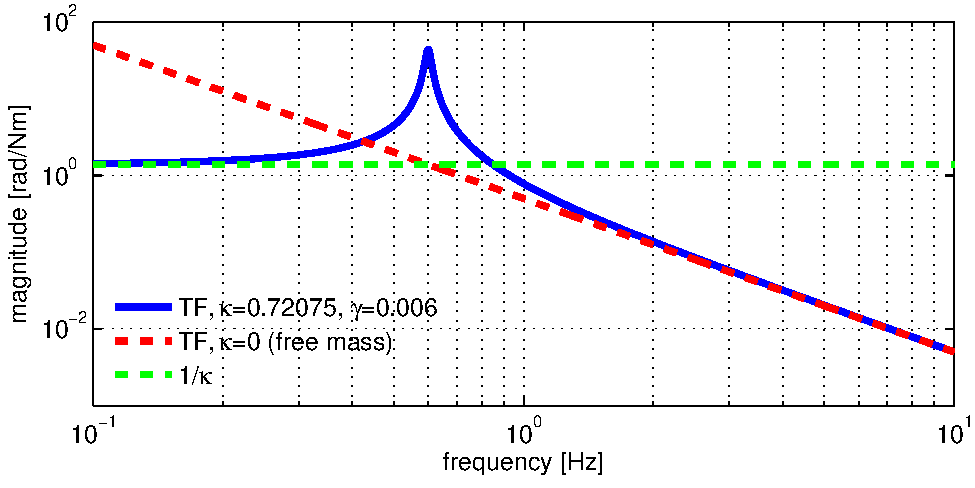
\includegraphics[width=1.0\textwidth]{figures/pendTF.pdf}
\caption[Torque to pitch transfer function of a LIGO core
optic]{Torque to pitch transfer function of a LIGO core optic
  (blue). The optic acts like a free mass at high frequencies (red)
  and the DC magnitude of the transfer function is determined by the
  inverse torsional constant (green). A damping constant $\gamma =
  0.006$ ($Q=32$) was selected for pictorial representation only. The
  resonant frequency of LIGO core optics in yaw is 0.5~Hz.}
\label{fig:pendTF}
\end{centering}
\end{figure}





\section{Overview of Interferometer Alignment}
\label{sec:alignment_overview}

There are 8 mirrors whose pitch and yaw angles must be sensed and controlled. The sensing is accomplished by 8 sensors, which fall into three groups:
\begin{itemize}
\item camera image (BS): senses the position of the beam on the BS \vspace{-10pt}
\item quadrant photodiodes (QPDX, QPDY): sense the position of the light transmitted through the ETMs \vspace{-10pt}
\item wavefront sensors (WFS1, WFS2\footnote{Two signals are derived from WFS2.}, WFS3, WFS4): sense the angular misalignment of the cavities with respect to their input beams
\end{itemize}
Figure~\ref{fig:ASCsensors} shows the locations of these sensors and the 8 mirrors they must control. The alignment scheme can be simplified by considering it in two basic units: the input beam and the power-recycled Fabry-Perot Michelson (FPM). The alignment of the latter is self-contained (with the exception of the BS) and uses the WFS to keep the mirrors aligned to one another from DC up to several Hz. The alignment of the input beam to the power recycled FPM unit is accomplished via the BS camera image and QPDX at frequencies well below the pendulum resonances. Finally, as part of the input beam alignment, QPDY keeps the beam that is reflected from the BS pointed at the y-arm. The alignment scheme is depicted in Figure~\ref{fig:ASClayout} and explained in more detail in the remainder of this section.

\begin{figure} 
\begin{centering} 
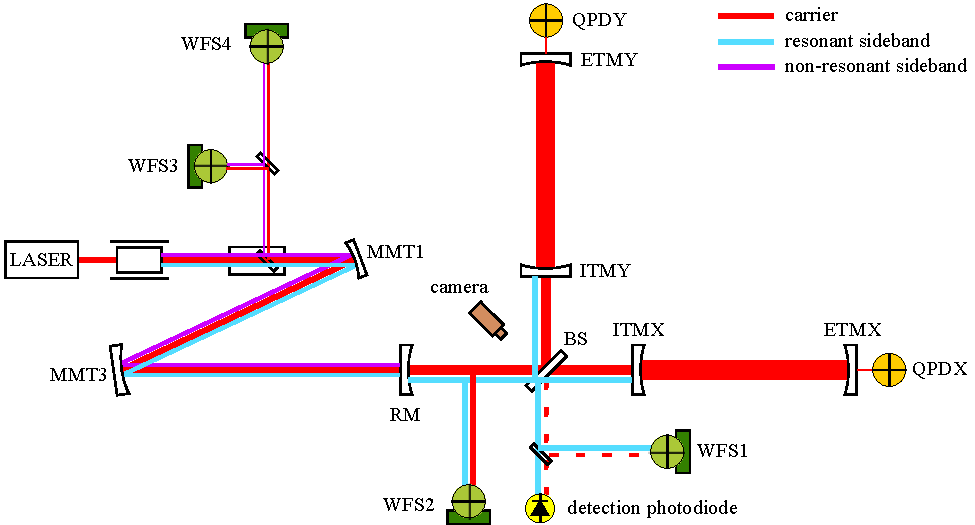
\includegraphics{figures/ASCsensors.pdf} 
\caption[Layout of ASC sensors and the mirrors they must control]{Layout of ASC sensors (WFS, QPDs, and camera) and the 8 mirrors they must control (ITMs, ETMs, MMTs, BS, and RM).}
\label{fig:ASCsensors}
\end{centering}
\end{figure}

\begin{figure} \begin{centering} \subfigure[]{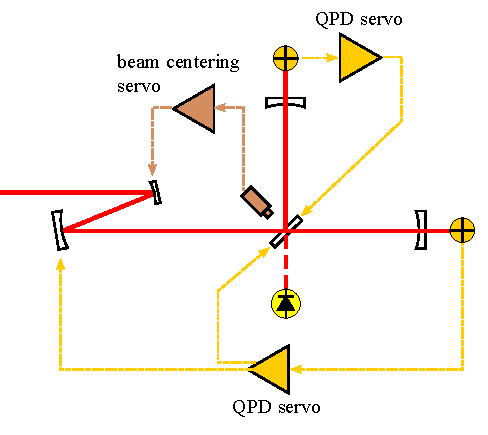
\includegraphics{figures/asc_inputctrl.pdf}}\subfigure[]{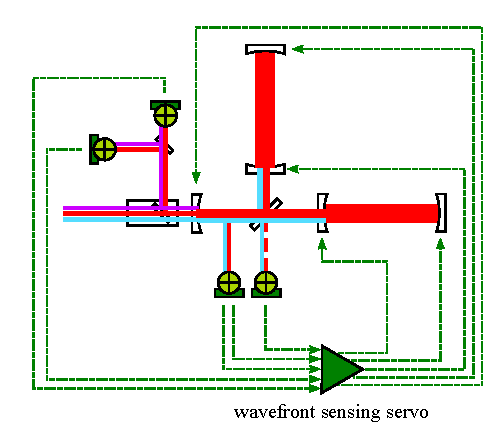
\includegraphics{figures/asc_PRFPMctrl.pdf}} \caption[Schematic of the alignment sensing and control system, viewed as two different units.]{Schematic of the alignment sensing and control system, viewed as two different units. A) The QPD servo and beam centering servo (BCS) together direct the input beam on minute time scales. B) The wavefront sensing servo maintains the alignment of the power-recycled FPM mirrors with respect to each other up to several Hz.}
\label{fig:ASClayout}
\end{centering}
\end{figure}

The self-contained alignment of the power-recycled Fabry-Perot Michelson is realized through the set of wavefront sensors (WFS)\footnote{Pronounced ``woofs''.} which provide the most sophisticated form of measuring angular motion of the mirrors and whose principle of operation is described in Section~\ref{sec:WFSsensing}.  The pitch and yaw motions of the five mirrors in this unit, ETMX, ETMY, ITMX, ITMY, and the PRM, are sensed by the pitch and yaw of five WFS signals, WFS1Q, WFS2I, WFS2Q, WFS3I, and WFS4I, where I and Q denote in-phase and quadrature demodulation, respectively. These WFS look at light at the AS port, at the reflected port, and in the power recycling cavity. Their error signals are used to control the relative motions of these five mirrors up to a couple Hz. The original design of wavefront sensing for a power-recycled Michelson with Fabry-Perot cavities in the arms was created and tested by Mavalvala \cite{Mavalvala1998Experimental, Mavalvala1997Alignment}.

The MMT-directed input beam and the power-recycled FPM unit need to be aligned to one another such that the input beam is perfectly reflected upon itself. Over minute time scales, the input beam follows the interferometer and over faster time scales the interferometer follows the input beam. This is achieved via a blend of all sensors. The low frequency matching of the input beam to the interferometer is realized through the pitch and yaw signals of QPDX, a QPD which monitors the position of the light transmitted through the x-arms, and the pitch and yaw signals of a camera that monitors the location of the beam spot on the beam splitter. These two alignment sensors adjust the pointing of MMT1 and MMT3 at about 30~mHz. The camera's beam centering servo (BCS) works by taking the image of the speckle of light reflected off of the beam splitter as shown in Figure \ref{fig:BCS} and feeding it into a labview program which integrates the intensity of the image to identify the coordinates of the center of the beam spot. These coordinates are compared with a hardcoded desired center location. A mirror upstream, MMT1, is moved to redirect the input beam, minimizing the difference between the desired and actual beam spot location on the BS. The QPD servos work in a similar fashion. The higher frequency matching of the input beam and the interferometer to one another is achieved by the reflected port wavefront sensors (WFS3 and WFS4), up to a couple Hz.

\begin{figure} 
\begin{centering} 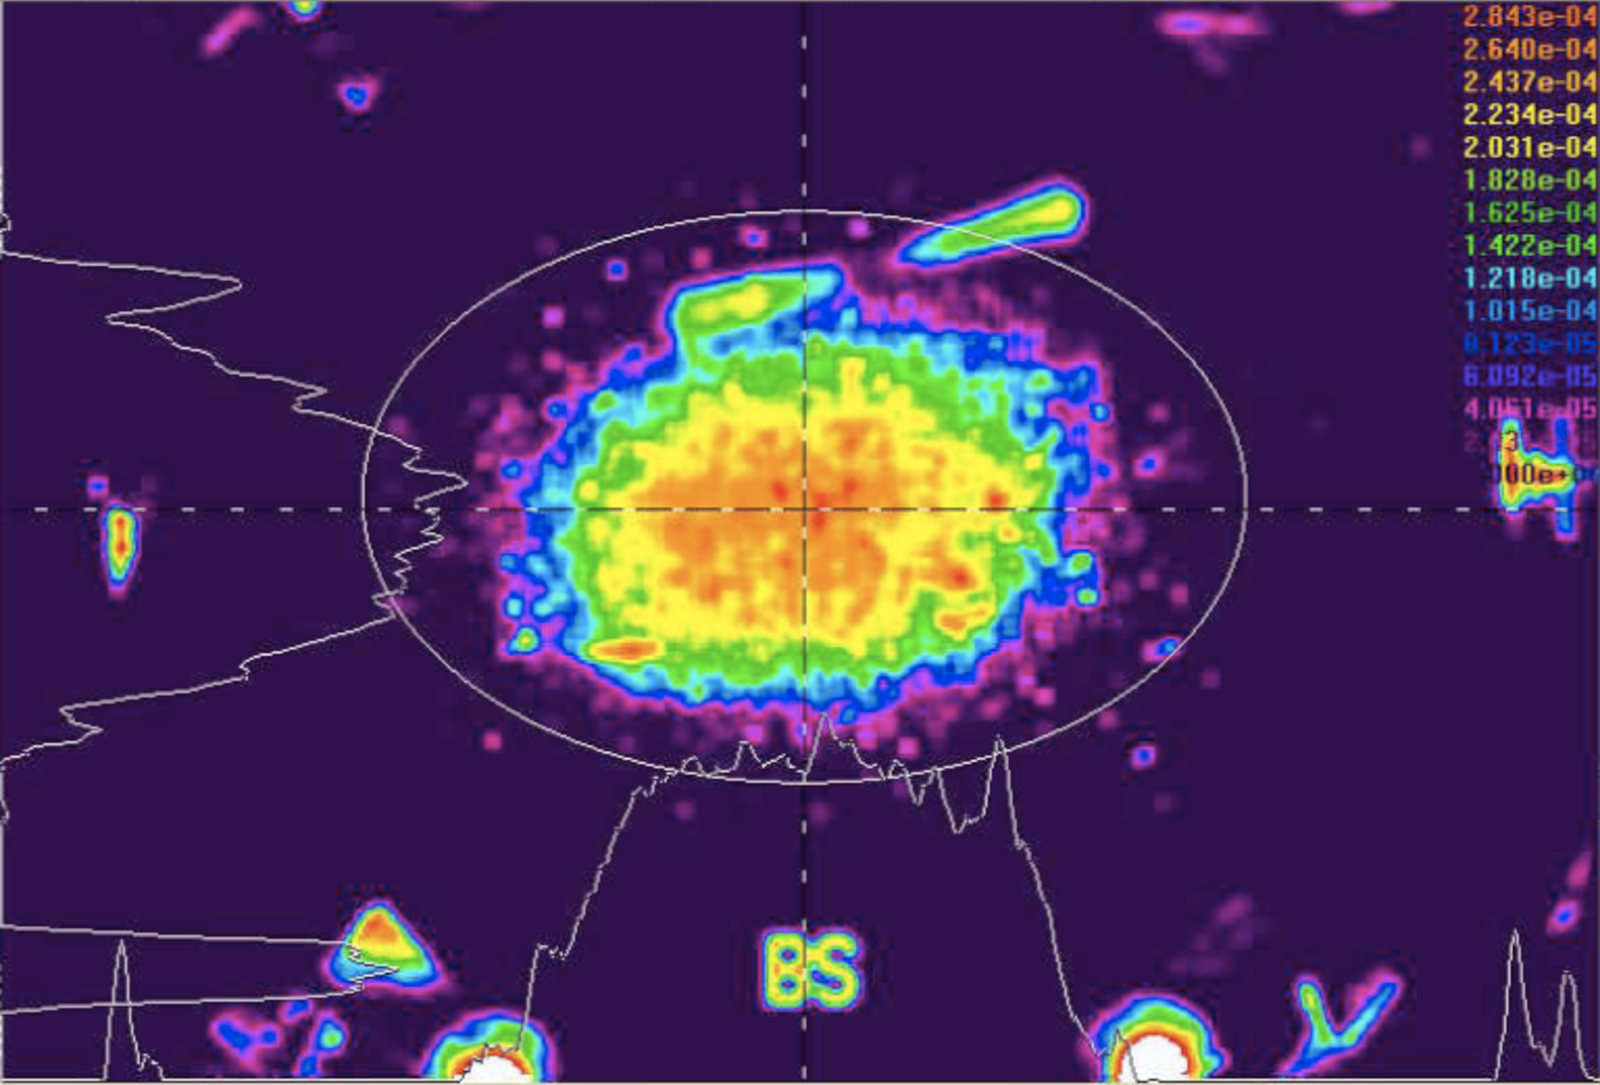
\includegraphics[width=0.7\textwidth]{figures/BCSspiricon.pdf} 
\caption[Beam centering servo image of beam splitter]{Image of beam on beam splitter as used in the beam centering servo. The beam appears stretched because the camera's viewing angle is at $45^{\circ}$ with respect to the mirror surface. The color scale is arbitrary, but orange is strong, violet is weak.}
\label{fig:BCS}
\end{centering}
\end{figure}

The one additional step needed for full interferometer alignment is to maintain the relative alignment of the y-arm to the x-arm as the x-arm and input beam together move around. This is accomplished through the pitch and yaw signals of QPDY, the QPD that monitors the light transmitted through the y-arm, which sense how the beam splitter should be pointed. QPDX also sends a signal to the BS to compensate for the signal it sends to MMT3.

All mirror angles are of course inter-dependent and they must track each other. However, a rough hierarchy of who follows who can be established because ultimately the interferometer is bolted to the ground and necessarily maintains some DC orientation. This orientation comes from QPDX and QPDY, which are physically attached to piers standing on the ground and force the beams transmitted through the ETMs to stay put at a certain location on their sensors. In all, the input beam must make it to those two exact places and the other mirrors are left to line themselves up accordingly. 

This alignment process involving the WFS, QPDs, and BS camera relies on the entire interferometer already being locked. It manages the continuous fine-tuning of mirror angles so that maximal power buildup in the interferometer is maintained, and so that the interferometer does not wander from its linear operating point (described in Section~\ref{sec:DCreadout}). How to achieve the initial alignment of all of the mirrors is an interesting process in itself and is documented in Appendix~\ref{sec:initial_alignment}.



\section{The Angular Sensing and Control Servo}
When the interferometer is locked, the optical levers and the wavefront sensors provide simultaneous feedback to the mirror angles. The optical levers provide local damping, and the WFS maintain both the alignment of the power-recycled FPM with the input beam and the internal alignment of the power-recycled FPM. The study and characterization of the elements of this angular control system when the laser power is increased is the topic of the remainder of this chapter and the next. First, it is helpful to present an overview of the servo without the effects of radiation pressure.

\begin{figure} \begin{centering} 
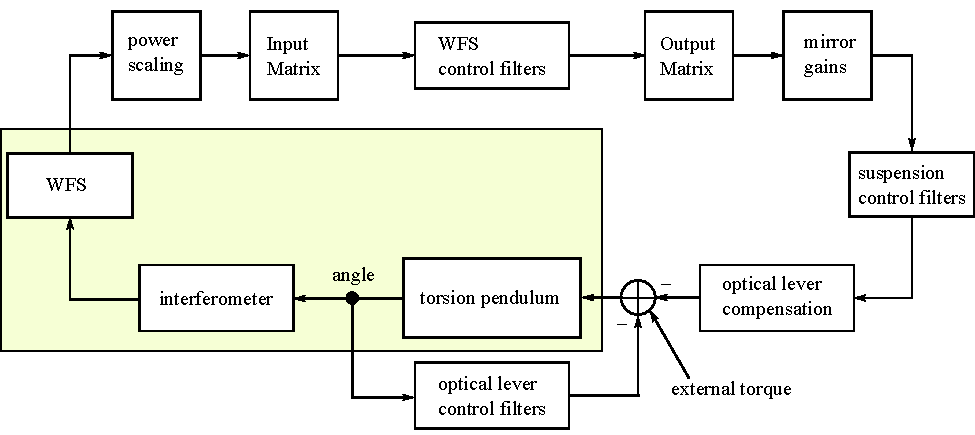
\includegraphics{figures/ASCcontrolservo.pdf} 
\caption[ASC control servo]{ASC control servo, showing both the WFS and optical lever loops. The external torque, torsion pendulum, interferometer, and WFS are analog; all other blocks are digital. Mirror angles are converted by the interferometer into signals the wavefront sensors can detect. These WFS error signals are digitized, filtered, and converted into analog control signals for individual mirrors. The details of each of the digital blocks are explained in Chapter~\ref{ch:characterization}.}
\label{fig:ASCcontrolservo}
\end{centering}
\end{figure}

Figure~\ref{fig:ASCcontrolservo} is a block diagram of the major components to the angular control servo. The torsion-like pendula of the interferometer are subject to external torque which is converted to mirror angle. The interferometer, in turn, turns the mirror angles into $\mathrm{TEM}_{10}/\mathrm{TEM}_{01}$ modes at its various ports, and these modes are converted into error signals by the wavefront sensors. The voltages produced by the wavefront sensors are digitized and manipulated by the front-end computers to create control signals that are then converted back to analog signals for actuation on the mirrors. The result of this process is a suppression of the error signal seen by the WFS and therefore a suppression of the physical relative mirror motions. 



\subsection{The Wavefront Sensing Scheme}
\label{sec:WFSsensing}
The wavefront sensors provide the most sophisticated form of measuring angular motion of the mirrors. They are quadrant photodiodes equipped with RF electronics that rely on the Pound-Drever-Hall locking scheme to produce error signals \cite{Sigg1996Wavefront}. WFS are the angular equivalent of the single element PDs used for length sensing. Their frame of reference is the fundamental Gaussian mode of the interferometer cavities; angular misalignments of the cavities generate TEM$_{01}$ and TEM$_{10}$ spatial modes of the carrier light as explained in Ref.~\cite{Anderson1984Alignment} and derived in Appendix~\ref{sec:cavitypower}. The overlap of the higher order mode carrier field with a TEM$_{00}$ reference sideband field produces an excess of power on one half of the detector compared to the other when demodulated at the sideband frequency. This is the error signal. The sidebands 

Reference \cite{Fritschel1998Alignment} contains a thorough description of the wavefront sensing scheme. In summary, the idea is that the WFS are located where optical gain, the amount of laser power produced at some interferometer port for a given physical change of some aspect of the interferometer, is high. The WFS optical gain in, particular, is determined by how much TEM$_{01}$/TEM$_{10}$ mode shows up at the locations of the WFS when a mirror (or specific combination of mirrors) moves in angle. One WFS is placed at the anti-symmetric port where differential-mode signals are transmitted, one is placed at a pick-off of the beam from the recycling cavity which contains common and differential information, and two are placed at the reflected port, where common-mode signals are transmitted. The precise locations are determined from the Gouy phases of the light and details are found in Ref.~\cite{Barsotti2009Modeling}.



\subsection{The Digital Path}
The digital portion of the servo, from the power scaling through the optical lever compensation, experiences two changes of basis which are effected by the input matrix and the output matrix. The input matrix takes the appropriate linear combination of WFS error signals to create error signals for which control filters may be designed easily. The output matrix creates a linear combination of the digital control signals in order to distribute them appropriately to specific mirrors. Both the power scaling and the mirror gains are diagonal matrices that provide minor modifications to the amplitude of the error and control signals, respectively. The power scaling is updated in real time to compensate for any changes in laser power on the WFS. The mirror gains are hard-coded scaling factors to reflect deviations from the theoretical cavity geometry. See Sections \ref{sec:powerscaling} and \ref{sec:mirrorgains}, respectively, for details.



\subsection{Optical Lever Compensation}

\begin{figure} 
\begin{centering} 
\subfigure[]{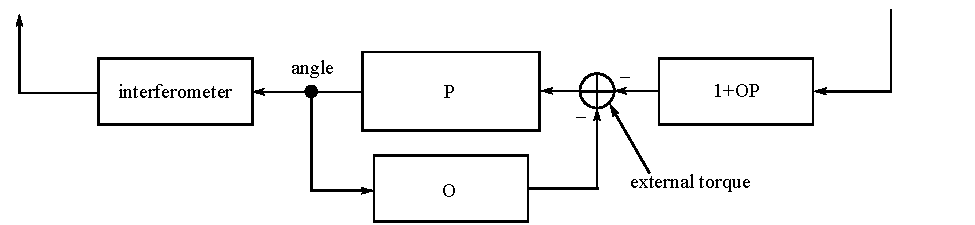
\includegraphics{figures/OLcompensation.pdf}} 
\subfigure[]{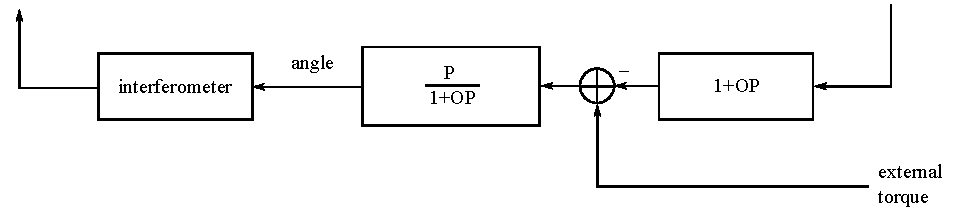
\includegraphics{figures/OLcompensation2.pdf}} 
\subfigure[]{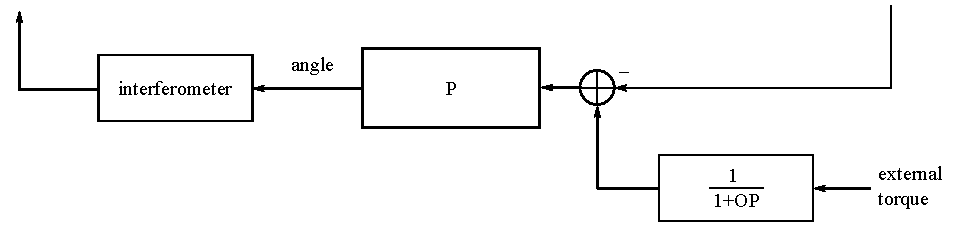
\includegraphics{figures/OLcompensation3.pdf}} 
\caption[Optical lever compensation scheme]{Optical lever compensation scheme. Subfigures A, B, and C are equivalent. A) Zoom of the bottom part of Figure~\ref{fig:ASCcontrolservo}. $P$ is the pendulum and $O$ is the optical lever digital control filters. B) Replacement of the optical lever controlled plant with the closed loop gain representation. C) Optical lever compensation removes the optical levers from the picture of the pendulum. External torque is still suppressed by the optical lever closed loop gain.}
\label{fig:OLcomp} 
\end{centering} 
\end{figure}

\label{sec:oplevcomp}
Each of the large optics has its own optical lever servo that provides velocity damping. Since both the WFS and the optical levers control the mirror motion when the interferometer is locked, we must consider the interaction of the two servos. Whether one views the interaction as the WFS controlling the optical-lever-controlled mirrors or as the optical levers controlling the WFS-controlled-mirrors is arbitrary. For the purpose of explanation here, I use the former viewpoint.

Figure \ref{fig:OLcomp} zooms in on the portion of the Figure \ref{fig:ASCcontrolservo} control loop picture that shows the optical lever controlling the pendulum. The torque to angle transfer function of the pendulum is our plant, $P$, the optical lever control is $O$, and the optical lever compensation is shown as $1+OP$. A result of basic control theory is that the optical lever controlled pendulum loop can be represented by its closed loop transfer function:
\begin{equation}
\mathrm{TF_{closed}} = \frac{P}{1+OP}
\end{equation}
as shown in Figure \ref{fig:OLcomp}~B. 

One will notice that it is not a coincidence that the optical lever compensation has the same form as the denominator of the closed loop transfer function. Together, they cancel each other out, and all that remains as the plant is the simple pendulum. Including the optical lever compensation in the ASC loop is not necessary, but it is a useful technique for simplifying the design process of the WFS control filters. One need only consider how to control the simple pendulum torque to angle transfer function, rather than the optical-lever controlled pendulum.

\begin{figure} \begin{centering} \subfigure{\includegraphics{figures/WFS1Q_darkres.pdf}}\subfigure{\includegraphics{figures/WFS2I_darkres.pdf}}\subfigure{\includegraphics{figures/WFS2Q_darkres.pdf}} 
\subfigure{\includegraphics{figures/WFS3I_darkres.pdf}}\subfigure{\includegraphics{figures/WFS4I_darkres.pdf}} 
\caption[WFS error signal and dark noise]{WFS dark noise compared to typical error signal. The excess signal above the dark noise in WFS3I and WFS4I above 20~Hz is likely acoustic noise, although this hypothesis has not been verified. WFS1 and WFS2 are on a floating table in a sound proof chamber, while WFS3 and WFS4 are on a non-seismically isolated table without a sound proof enclosure. Seismic noise at time of residual spectra is in Figure~\ref{fig:seismic_locked}.}
%\textcolor{blue}{Include shot noise, too, especially for WFS1.}
\label{fig:WFSdarknoise}
\end{centering}
\end{figure}



\section{Angular Control Limitations}
\label{sec:ASClimits}
The limits for how well we can control the angular motion of the interferometer are governed by how well we are able to sense the angular motion. Several of the wavefront sensors' signals are dark-noise-limited above 20-25~Hz, as seen in Figure \ref{fig:WFSdarknoise}. Moreover, depending on the power level, WFS1Q may instead be limited by shot noise (refer to Eq. \ref{eq:shotnoise}). Any control signal derived from frequencies in the sensing noise limited regime will impress the sensor noise on the mirrors. The impression of sensor noise cannot be avoided entirely in the presence of feedback, but can be mitigated by including amongst the control filters a steep cut-off beginning at frequencies where sensor noise dominates. 
%Ultimately, it is the WFS noise floor that determines the best possible achievable suppression. 

Besides the sensing noise, there are also sometimes real signals that result in more harm than good when used as feedback. The HAM seismic isolation tables used by the Input Optics (the core optics are suspended from BSC tables) have stack modes at 0.8 to 3~Hz that ring up the MMTs.  At low frequencies, around 1~Hz, some of the WFS signals are dominated by these angular fluctuations of the input beam. The resulting attempt of the mirrors to follow the input beam jitter leads to a magnification of the motion because of the drastically different length scales. Large power fluctuations in both arms and the power recycling cavity ensue, leading to departure from the linear error signal regime and often lock loss. 

Other limitations to the reduction of mirror motion result from the nature of control loops. The cut-off filter, for example, reduces the phase margin of the open loop gain, necessarily pushing down the unity gain frequency (UGF) and therefore the magnitude of suppression at all frequencies below the UGF. A less aggressive cut-off filter, while improving the servo's stability and allowing for higher overall gains, leads to more impression of sensing noise on the optics. Also, if the phase margin of the loop is low, mirror motion will be amplified through gain peaking.

% A final point that should be noted, but is in fact insignificant, is a coupling from angular drive to length that results from the same principle of the length to angle coupling presented in \ref{sec:L2A}. 

% We will show that we don't quite meet all of these requirements and the impression of sensing noise in fact plays a major role in the reduction of DARM sensitivity up to 70 Hz.



